 %% Präambel
\documentclass[
	11homerhopt,
	a4paper,
	oneside, 
	liststotoc, 					% Tabellen- und Abbildungsverzeichnis ins Inhaltsverzeichnis
	bibtotoc,						  % Literaturverzeichnis ins Inhaltsverzeichnis aufnehmen
	titlepage, 						% Titlepage-Umgebung statt \maketitle
	headsepline, 					% horizontale Linie unter Kolumnentitel
]{scrreprt}


\usepackage[english]{babel} 		% deutsche Trennungsregeln und Übersetzung der festcodierten Überschriften
\usepackage[T1]{fontenc} 			% Ausgabe aller zeichen in einer T1-Codierung (wichtig für die Ausgabe von Umlauten!)
\usepackage{graphicx}  				% Einbinden von Grafiken erlauben
\usepackage{textcomp} 				% zum Einsatz von Eurozeichen u. a. Symbolen
\usepackage{listings}				% Datstellung von Quellcode mit den Umgebungen {lstlisting}, \lstinline und \lstinputlisting
\usepackage[dvipsnames, table]{xcolor} 			% einfache Verwendung von Farben in nahezu allen Farbmodellen
\usepackage[intoc]{nomencl} 		% zur Erstellung des Abkürzungsberzeichnisses
\makenomenclature					% Abkürzungsverzeichnis erstellen
\usepackage{setspace}				% Zusatzpaket zur Einstellung des Zeilenabstands
\usepackage{longtable}
\usepackage{multirow}
 
\usepackage[lmargin=2.5cm, rmargin=2.5cm,tmargin=2.50cm,bmargin=2.50cm]{geometry}		% Seitenrändekr formatieren
\usepackage[style=alphabetic,citestyle=alphabetic,backend=bibtex]{biblatex}
\addbibresource[]{bib/bibtex.bib}

\usepackage{url}
\usepackage{eurosym}
\usepackage{amssymb}
\usepackage{amsmath}
\usepackage{amsthm}
\usepackage{todonotes}

% Fonts
%\usepackage{courier}
\usepackage[scaled]{beramono} % script font
\usepackage{caption}  % adapted captions
\usepackage{textcomp} % straight single quotess

% Check mark and cross mark
\usepackage{pifont}
\newcommand{\cmark}{\ding{51}}%
\newcommand{\xmark}{\ding{55}}%

% Table
\usepackage{booktabs}
\usepackage{arydshln}
\renewcommand{\arraystretch}{1.2}

\setlength{\nomlabelwidth}{.20\hsize}

% -----------------------------------------------------------------------------------------------------------------
% Zum Aktualisieren des Abkürzungsverzeichnisses bitte auf der Kommandozeile folgenden Befehl aufrufen :
%  makeindex Bachelorarbeit.nlo -s nomencl.ist -o Bachelorarbeit.nls
% -----------------------------------------------------------------------------------------------------------------

\definecolor{grey}{RGB}{050,050,050}
\definecolor{lightblue}{RGB}{224,238,238}
\definecolor{lightgrey}{RGB}{240,240,240}
\definecolor{darkgray}{rgb}{.4,.4,.4}
\definecolor{js_grey}{HTML}{778899}
\definecolor{js_blue}{HTML}{0077AA}
\definecolor{js_red}{HTML}{DD4A68}
\definecolor{js_green}{HTML}{669900}


\newcommand{\tab}{\qquad \qquad \qquad \qquad \qquad \qquad \qquad}
\setlength{\parindent}{0em}  	% Absatzeinrückung eliminieren

% ------------------------------ Persönliche Daten ------------------------------------------

\newcommand{\thesisTitle}{Application Security}
\newcommand{\thesisSubtitle}{Investigation and Validation of NoSQL Injection Vulnerabilities}
\newcommand{\work}{Master Thesis}
\newcommand{\studyCourse}{Computer Science}
\newcommand{\auth}{Patrick Spiegel}
\newcommand{\studendNumber}{1854488}
\newcommand{\deadline}{\today}
\newcommand{\period}{09. Mai - 08. November 2016}
\newcommand{\professor}{Prof. Dr. J\"orn M\"uller-Quade}
\newcommand{\professorTwo}{Prof. Dr. Dennis Hofheinz}
\newcommand{\companySupervisor}{Dr. Martin Johns}

% ------------------------------ Befehle ----------------------------------------------------
\newcommand{\jahr}{2016}			% für Angabe im Copyright-Vermerk der Titelseite

\newcommand{\changefont}[3]{\fontfamily{#1} \fontseries{#2} \fontshape{#3} \selectfont}

% ------------------------------ Abkürzungen ------------------------------------------------
\newcommand{\ua}{\mbox{u.\,a.\ }}
\newcommand{\zB}{\mbox{z.\,B.\ }}
\newcommand{\bs}{$\backslash$}

% ------------------------------ Titeländerungen --------------------------------------------
\renewcommand{\nomname}{List of Abbreviations}
\renewcommand{\lstlistlistingname}{List of Listings}

% -------------------------------------------------------------------------------------------
% Design von Listings
% -------------------------------------------------------------------------------------------
\definecolor{lighter-gray}{RGB}{244,244,244}
\lstset{
  %frame=top,frame=bottom,
  backgroundcolor = \color{lighter-gray},
  basicstyle=\ttfamily\footnotesize,    % the size of the fonts that are used for the code
  stepnumber=1,                           % the step between two line-numbers. If it is 1 each line will be numbered
  numbersep=10pt,                         % how far the line-numbers are from the code
  tabsize=2,                              % tab size in blank spaces
  extendedchars=true,                     %
  breaklines=true,                        % sets automatic line breaking
  captionpos=b,                           % sets the caption-position to top
  stringstyle=\color{blue}\ttfamily, % Farbe der String
  showspaces=false,           % Leerzeichen anzeigen ?
  showtabs=false,             % Tabs anzeigen ?
  xleftmargin=17pt,
  framexleftmargin=17pt,
  framexrightmargin=17pt,
  framexbottommargin=2pt,
  framextopmargin=2pt,
  showstringspaces=false,
  numbers=left,
  numberstyle=\tiny,
  upquote=true
}

\DeclareCaptionFormat{listing}{\vskip1pt#1#2#3}
\captionsetup[lstlisting]{format=listing,singlelinecheck=false, margin=0pt, font={small,sf},labelsep=space,labelfont=bf}
\captionsetup[figure]{format=listing,singlelinecheck=false, margin=0pt, font={small,sf},labelsep=space,labelfont=bf, justification=centering}
\captionsetup[table]{format=listing,singlelinecheck=false, margin=0pt, font={small,sf},labelsep=space,labelfont=bf, justification=centering}

\lstdefinelanguage{JavaScript}{
  keywords={typeof, new, true, false, catch, function, return, null, catch, switch, var, if, in, while, do, else, case, break},
  keywordstyle=\color{js_blue}\bfseries,
  ndkeywords={class, export, boolean, throw, implements, import, this, delete},
  ndkeywordstyle=\color{js_green}\bfseries,
  identifierstyle=\color{black},
  sensitive=false,
  comment=[l]{//},
  morecomment=[s]{/*}{*/},
  commentstyle=\color{js_grey}\ttfamily,
  stringstyle=\color{js_red}\ttfamily,
  morestring=[b]',
  morestring=[b]"
}

% -------------------------------------------------------------------------------------------
% Definition of Abbreviation-file 
% -------------------------------------------------------------------------------------------
\nomenclature{SQL}{Structured Query Language}
\nomenclature{NoSQL}{Not only Structured Query Language}
\nomenclature{HTTP}{Hypertext Transfer Protocol}
\nomenclature{HTTPS}{Hypertext Transfer Protocol Secure}
\nomenclature{DoS}{Denial of Service}
\nomenclature{CSRF}{Cross-site Request Forgery}
\nomenclature{PHP}{PHP Hypertext Preprocessor}
\nomenclature{URI}{Uniform Resource Identifier}
\nomenclature{SOAP}{Simple Object Access Protocol}
\nomenclature{WSDL}{Web Services Description Language}
\nomenclature{ACID}{Atomicity, Consistency, Isolation, Durability}
\nomenclature{JSON}{JavaScript Object Notation}
\nomenclature{BSON}{Binary JavaScript Object Notation}				% Datei mit Abkürzungen laden

% ------------------------------ Hyperref ------------------------------------------
\usepackage{hyperref}
\hypersetup{
    bookmarks=true,         % show bookmarks bar?
    unicode=false,          % non-Latin characters in Acrobat’s bookmarks
    pdftoolbar=true,        % show Acrobat’s toolbar?
    pdfmenubar=true,        % show Acrobat’s menu?
    pdffitwindow=false,     % window fit to page when opened
    pdfstartview={FitH},    % fits the width of the page to the window
    pdftitle={\thesisSubtitle}, % title
    pdfauthor={\auth},      % author
    pdfsubject={\work},     % subject of the document
    pdfcreator={\auth},     % creator of the document
    pdfproducer={\auth},    % producer of the document
    pdfkeywords={keyword1, key2, key3}, % list of keywords
    pdfnewwindow=true,      % links in new PDF window
    colorlinks=false,       % false: boxed links; true: colored links
    linkcolor=red,          % color of internal links (change box color with linkbordercolor)
    citecolor=green,        % color of links to bibliography
    filecolor=magenta,      % color of file links
    urlcolor=cyan           % color of external links
}

% -------------------------------------------------------------------------------------------
%                     Beginn des Dokumenteninhalts
% -------------------------------------------------------------------------------------------
\begin{document}
\setcounter{secnumdepth}{3}				% Nummerierungstiefe fürs Inhaltsverzeichnis
\setcounter{tocdepth}{3}					% Tiefe des Inhaltsverzeichnises
\changefont{cmr}{m}{n}						% Schriftart definieren

% ------------------------------ Titelei -----------------------------------------------------
\thispagestyle{plain}
\begin{titlepage}
\enlargethispage{4.0cm}
%\sffamily 								% Serifenlose Grundschrift für die Titelseite einstellen

\begin{minipage}[hbt]{10cm}
	\textbf{Institut f\"ur Theoretische Informatik} \\
  Arbeitsgruppe Kryptographie und Sicherheit \\

  \professor \\
  \professorTwo \\
\end{minipage}
\hfill
\begin{minipage}[hbt]{8cm}
  
\includegraphics[scale=.8]{images/logo_kit.pdf}
\end{minipage} \\ [16ex]


\begin{center}
\huge{\textsc{\textbf{\thesisTitle}}}\\[3ex]
\LARGE{\textbf{\thesisSubtitle}}\\[10ex]
\textcolor{grey}{
	\LARGE{\textbf{\work\\[1ex]}}
	\Large{of \studyCourse}\\[1ex]
	by\\[2ex] \LARGE{\textbf{\auth}} 
} \\[18ex]


\end{center}

\begin{flushleft}

\begin{tabular}{ll}
Date:					& \tab \deadline \\ [1ex]
Period of processing:			& \tab \period   \\ [1ex]
Matriculation number: 			& \tab \studendNumber \\ [1ex]
\\
Primary Reviewer: & \tab \professor \\ [1ex]
Secondary Reviewer: & \tab \professorTwo \\ [1ex]
Company Supervisor:  & \tab \companySupervisor \\ [1ex]

\end{tabular} 



\end{flushleft}

\end{titlepage} 				% erzeugt die Titelseite

\pagenumbering{Roman}             % große, römische Seitenzahlen für Titelei
\begin{onehalfspace}
  \addchap{Statement of Authorship}
I declare that I have developed and written the enclosed thesis completely by myself, and have not used sources or means without declaration in the text.
\\[10ex]

\underline{\hspace{6cm}} \newline
Karlsruhe,  \deadline \\[4ex]


 				% Einbinden der eidestattlichen Erklärung
  \chapter*{Abstract} %*-mark to no appear in the contents listing
   				% Einbinden des Abstracts
\end{onehalfspace}
\tableofcontents							% Erzeugen des Inhalsverzeichnisses
\listoffigures 								% Erzeugen des Abbildungsverzeichnisses 
\listoftables 								% Erzeugen des Tabellenverzeichnisses
\lstlistoflistings

\printnomenclature							% Erzeugen des Abkürzungsverzeichnisses
% pdflatex - pdflatex - cmd: makeindex filename.nlo  -s nomencl.ist -o filename.nls        - pdflatex
\pagebreak

% --------------------------------------------------------------------------------------------
%                    Inhalt der Bachelorarbeit
%---------------------------------------------------------------------------------------------
\pagenumbering{arabic}              % arabische Seitenzahlen für den Hauptteil
\begin{onehalfspace}                % Zeilenabstand einstellen

  \chapter{Introduction}
\label{cha:introduction}
This first chapter outlines the underlying motivation for the investigation of NoSQL injection, defines the objectives in scope of this work and gives a look forward to the achieved academic contributions. Lastly, the structure of the thesis is elucidated.

\section{Motivation}
In the last decade many new challenges, such as big data, social media and the internet of things, changed the way we build applications. More and more devices got connected to the internet and started producing huge amounts of unstructured data. This new situation demanded for highly scalable, always available systems for large numbers of concurrent and globally distributed users. The by then prevailing relational databases did not meet the upcoming requirements and reached their limits facing the enormous amounts of data. Given these circumstances, the generation of NoSQL databases emerged. With a non-relational approach in common, these databases provided a solution for the given challenges. Flexible handling of unstructured and semi-structured data originating from different sources in combination with powerful horizontal scaling abilities lead to the break through of NoSQL technologies. Since then, these databases were deployed in many application stacks and serve millions of users every day. Google uses NoSQL solutions as a part of their compute engine \cite{MongoDB_Google:2016}, Facebook adapted its storage engine for NoSQL integration \cite{MongoDB_Facebook:2016} and SAP selected NoSQL technologies for the core content management of its PaaS offering \cite{MongoDB_SAP:2016}. These and many more examples leave no doubt that this new generation of databases offers notable advantages for modern applications, but do they provide security? When innovative concepts find their way to production, the security aspect is often neglected. Especially a well-known attack vector against relational databases - SQL injection - was not taken into account for NoSQL applications. Regarding injection, the prevalent opinion is that we are not building queries from strings, so we do not have to worry about injection vulnerabilities. This attitude may rest upon the few known attack vectors for NoSQL injection against specific platforms. However, the launch of the social media platform Diaspora showed that NoSQL injection is an serious issue \cite{McKenzie:2010}. This raises the question, whether the known examples were individual cases or NoSQL injection presents a general threat for our modern applications. Since NoSQL comprises a variety of databases with slightly different concepts and query languages, a versatile attack surface for injection is given. All the same time, only little effort has been made to discover potential injection vulnerabilities. On account of this prevailing situation, the subject of NoSQL injection has to be investigated comprehensively and in greater detail.

\section{Objective}
\label{sec:objective}
This thesis aims to give an encompassing overview of injection attacks against NoSQL databases. A precise understanding of a system's architecture is vital to analyze potential risks. NoSQL injection presents a relatively new and unexplored kind of attack. Therefore, a clear definition of the class of attacks has to be made. Since NoSQL technologies lead to changes of typical system structures, also the existing attacker models have to be reevaluated. The first objective of this thesis covers these subjects: \\

\textbf{Objective 1:} \textit{Detailed definition of NoSQL injection and the corresponding attacker models.} \\

Outgoing from these definitions concrete injection vulnerabilities in NoSQL databases has to be searched. Previous studies concentrated on single databases in combination with a specific application layer. In contrast to these published attack vectors, a more holistic approach is needed in order to give a widespread overview of the topic. On that account the most prevalent NoSQL technology stacks have to be selected and investigated with regard to injection vulnerabilities. For this reason, the second objective of this work is defined as follows: \\

\textbf{Objective 2:} \textit{Investigation of a selected group of NoSQL technology stacks for injection vulnerabilities regarding the defined attacker models.} \\

With the results of the investigation the vulnerabilities examined for their underlying problems. A differentiation between conceptional and implementation problems is an important aspect of this step. Vulnerabilities originating from implementation flaws can easily be fixed when reported, whereas conceptional problems are hard to solve in most cases. Conceptional vulnerabilities are based on the underlying design of the database. Therefore, the third objective covers the classification as follows: \\

\textbf{Objective 3:} \textit{Classification of known and found NoSQL injection vulnerabilities according to the underlying design problem.} \\

Based on the exposed design problems, the prevention of NoSQL injection attacks can be approached. An appropriate prevention mechanism should be able to reliably stop potential injection attacks, but all the same avoid false positives breaking existing applications. Thereby, a mitigation technique should require a reasonable amount of code changes and engineering effort. The final objective of this thesis is therefore set in the following way:\\

\textbf{Objective 4:} \textit{Elaboration of an approach for NoSQL injection mitigation addressing the underlying design problems.} \\

% and mitigation
The elaboration of these four objectives should allow a general overview of NoSQL injection and provide an outline of the threads modern applications have to face with this class of attacks. \\


\section{Contributions}

The main contributions of this thesis concerning NoSQL application security are:
\begin{description}
\item [Injection Attacks] NoSQL injection vulnerabilities are not a database oder application layer specific problem. Therefore, this thesis reveals new injection vectors for multiple NoSQL databases in combination with common application layers. With this broad range of investigated technology stacks, it is shown, that NoSQL injection is a general issue across non-relational databases.
\item [Attacker Models] Despite parallels to SQL injection attacks, the existing attacker models are not sufficient considering NoSQL injection. Since NoSQL databases are created with the aim to handle huge amounts of unstructured data from several sources, format restrictions are low. These circumstances may allow insertions of attacker controlled data from external sources. On account of this, an additional attacker model is introduced and exemplary attacks are presented to cover these new conditions.
\item [Injection Prevention] The mitigation of NoSQL injection is hard to ensure, since the data and therefore the requests assume various shapes across databases. In order to reduce the risk of injection attacks, this thesis breaks down known injection vectors to the underlying design problems. On basis of these a new database driver design is presented, that is resistant to known injection attacks.
\end{description}

\section{Structure}
This thesis is  structured as follows: In chapter two an overview of fundamental technologies of the thesis is given. Used protocols, investigated databases and the necessary security topics are outlined in this part. Chapter three gives an introduction to the concept of NoSQL injection as well as corresponding attacker models. Subsequently, the in scope of this thesis discovered injection vectors are presented in chapter four. A diverse technology stacks are addressed in this part. Chapter five classifies the found attack vectors based on their underlying problem. Based on this classification, chapter six presents a new approach for NoSQL injection mitigation. Within chapter seven, the presented solution is evaluated with real world applications. A comparison of this thesis to related publications is given in chapter eight. The last part, chapter nine, discusses the results of this thesis and gives a potential outlook for future work on the subject of NoSQL injection.
   \chapter{Technical Background}
\label{cha:technicalBackground}
This chapter outlines the essential technologies and techniques in the context of NoSQL injection. Thereby, the relevant fundamentals in the scope of this thesis are covered.

\section{Underlying Technologies}
Within this section, the prevalent protocols and paradigms for data exchange between systems are explained.

\subsection{HTTP}
The Hypertext Transfer Protocol (HTTP) represents an application-layer protocol for the transfer of connected multimedia documents \cite{Berners-Lee1996}\cite{Fielding:1999}. Initially, HTTP was created regarding web-server to web-browser communication, but today the protocol is applied for various purposes. As a stateless protocol following a client-server model, HTTP itself does not retain any state between requests. While the protocol is often applied as a part of the TCP/IP stack, it is also applicable with other reliable and error-checked protocols on the transport layer. A required header block and an optional body block build the basic structure of each request and response. Depending on the intended kind of operation, different methods for requests exist. Table \ref{tab:http_methods} gives an overview of the available HTTP methods and their characteristics.\\

\begin{table}[h] 
 \centering
 \begin{tabular}{llccc}
  \textbf{\begin{tabular}{@{}c@{}}HTTP \\ method\end{tabular}} & \textbf{Description} & \textbf{\begin{tabular}{@{}c@{}}Request \\ body\end{tabular}} & \textbf{\begin{tabular}{@{}c@{}}Response \\ body\end{tabular}} & \textbf{Idempotent} \\ \hline
  GET     & Retrieve specified resource & \xmark & \cmark & \cmark \\
  HEAD    & Retrieve specified resource headers & \xmark & \xmark & \cmark \\
  POST    & Create specified resource & \cmark & \cmark & \xmark \\
  PATCH   & Partially updated specified resource & \cmark & \cmark & \xmark \\
  PUT     & Replace specified resource & \cmark & \cmark & \cmark \\
  DELETE  & Delete specified resource & \xmark & \cmark & \cmark \\ \midrule
  CONNECT & Convert connection to tunnel & \cmark & \cmark & \xmark \\
  OPTIONS & Return supported HTTP methods & \cmark & \cmark & \cmark \\
  TRACE   & Echo received request & \xmark & \cmark & \cmark \\
  \bottomrule
 \end{tabular}
 \caption{Overview of HTTP methods' characteristics}
 \label{tab:http_methods}
\end{table}

Basically, the first six methods implement create, read, update and delete operations for resources on the server. Thereby, a URI in the header specifies the resource, that the operation should be applied to. In case of create or update operations, the optional body block in the request contains the new resource data. Since no new data is needed for resource retrieving and deleting methods, they work solely with the request header block. All operations, apart form the HEAD request, deliver the result of the operation within the response's body block. Idempotents indicates, whether the behavior of a method stays the same for multiple consecutive requests. Especially update operations do not feature idempotent characteristics. The last three methods represent helper functions for connection inspection and TCP tunneling. An example for a request, that retrieves a specified resource form the server, is given in listing \ref{lst:http_request}.

\begin{lstlisting}[caption={HTTP GET request}, label={lst:http_request}]
GET /index.html HTTP/1.1
Host: example.org
Accept-Language: en
\end{lstlisting}

The first line of the request header is composed of the HTTP method, followed by resource identifier and completed with the version of the used protocol. In the given example a  GET request is used in order to retrieve the \textit{index.html} file. Afterwards, the host of the server is defined by the domain name. Accepted types of files, char-sets, encodings, languages and many more settings can be defined as additional headers. In case the requested resource exists and no error appears during request processing, the server sends a response as exemplified in listing \ref{lst:http_response}.

\begin{lstlisting}[caption={HTTP GET response}, label={lst:http_response}]
HTTP/1.1 200 OK
Date: Sat, 09 Sep 2016 14:28:02 GMT
Server: Apache
Last-Modified: Tue, 01 Dec 2009 20:18:22 GMT
ETag: "51142bc1-7449-479b075b2891b"
Accept-Ranges: bytes
Content-Length: 29769
Content-Type: text/html

<!DOCTYPE html... (here comes the 29769 bytes of the requested web page)
\end{lstlisting}

In the first line of the response, the server version of the protocol as well as the status code and message are returned. Depending on the success of the request, the status code and message in the response change. Further headers contain meta information about the server, the requested resource and the body block. Separated by a blank line, the body block follows the header. In this example the body contains the requested HTML document. With the end of the response body, the HTTP request-response cycle is finished.

\subsection{REST}
Representational State Transfer (REST) describes a programming paradigm for distributed systems in a stateless client-server environment \cite{Fielding:2000}. It specifies an architectural style, that enforces a consistent system interface design. Therefore, REST represents an alternative to prior approaches, such as SOAP or WDSL. The paradigm separates resource location and the applied method. Functional instructions are therefore not allowed to be included within the URI. A special implementation or protocol is not defined by the paradigm, whereby REST is commonly used in combination with HTTP and HTTPS. In the course of this, the HTTP methods encode the functional instructions and resources has to be uniquely identified by the requested URI. Though, the usage of HTTP and HTTPS does not imply REST conformance. Methods are often misused for different functionalities and as a result REST conformance is not provided.

\section{NoSQL Databases}
This section gives an introduction to NoSQL databases and the idea behind this new class of data storage. NoSQL databases and their concepts, that are relevant in scope of this work, are outlined in detail.

\subsection{Overview}
In 1998 the word \textit{NoSQL} was first used by Carlo Strozzi in context of a relational, document-oriented database designed to be accessed without SQL. More than 10 years later in 2009, Johan Oskarsson reintroduced the term \textit{NoSQL} in oder to find a collective name for the increasing number of distributed, non-relational databases. From this time forward, the term was used with the meaning of \textit{not only SQL} or \textit{non relational} instead of \textit{no SQL}. Therefore, the term builds an umbrella term for databases without relational restrictions and often missing ACID support. The idea for such databases arose back in the 1960s, but the actual trend started with the challenges of big data. NoSQL databases addressed these challenges through their flexible data models, distributed storage, horizontal scaling abilities and independence from dedicated hardware. Currently around 225 databases are prevalent, that denote themselves as NoSQL storage. Despite the shared non-relational concept, NoSQL databases can be divided in different categories. Depending on the focused field of application, there exist four major groups:

\begin{description}
\item [Key-value Stores] These databases reference datasets with unique keys. Datasets are accessed with the key, that retrieves a pointer to the dataset from a hash table. Therefore data access over the key is very fast, but querying or updating single properties of a dataset is inefficient. Notable examples for key-value stores are Redis, Riak, Voledmort or Memcached.
\item [Document Stores] The main idea here is similar to key-value stores, but datasets also are composed of semistructured key-value pairs. These datasets are often called documents and are persisted in formats like JSON. This allows more efficient querying for single properties of a dataset. Notable examples for document stores are MongoDB, CouchDB or CouchBase.
\item [Graph databases] This group uses a flexible structure with nodes and edges to model graph structures. Depending on the implementation and the underlying data persistence, the data access differs. Some databases implement RESTful interfaces, others provide dedicated query APIs. Notable examples for graph databases are Neo4j, Titan or Graphite.
\item [Column Stores] Similar to relational databases, data is very structured, but the underlying persistence layer differs strongly. Data is arranged column after column instead of row after row. This column oriented storage allows the processing and especially analysis of large amounts of data over distributed systems. Notable examples for column stores are Apache Cassandra, HBase or SAP HANA.
\end{description}

Apart from the presented categories of NoSQL databases, there also exist hybrid models implementing features originating from multiple categories. An example is OrientDB, that combines a document store with graph database abilities. 

\subsection{MongoDB}
The non-relational, document-oriented database MongoDB was published as an open-source project in 2009. Deriving its name from the word humongous, it is designed to provide high performance, high availability as well as automatic horizontal scaling. The JSON style data model enables complex hierarchies for stored documents, but still allows efficient querying and indexing. Documents are stored in Binary JSON (BSON) format into collections, that in turn can be queried by JSON expressions. BSON extends JSON with additional data types, such as date, time stamps and regular expressions and is binary encoded. By default every MongoDB instance holds special system collections for indexes, namespaces, users and JavaScript code. MongoDB provides official drivers for various popular programming languages next to many unofficial community-supported drivers. 

\subsection{Redis}
Redis is an in-memory operating key-value store for strings, hashes, lists and sets. The 2009 released open-source database allows range queries and has built in Lua support for scripting. Due to its low data structure complexity, Redis provides large performance advantages in comparison to relational databases. Snapshotting or append only files allow on-disk persistence of the in-memory stored data. Later versions also allow distributed storage across clusters. Redis provides driver bindings for the most prevalent programming languages.

\subsection{Memcached}
The in 2003 released database Memcached is an in-memory key-value store for data caching. It allows to store and retrieve data from memory with hash tables distributed across multiple systems. Therefore, the result of requests to external sources can be cached and accessed much faster for subsequent access. Since the database is designed as a cache, data persistence on disc is not provided by default. Due to the resulting performance benefits of this approach, Memcached achieved wide prevalence and is deployed by companies like Facebook, YouTube, Twitter and Wikipedia. Drivers are provided for all major programming languages.


\subsection{CouchDB}
CouchDB is an document-oriented database written in Erlang. First published in 2005, the database is now maintained by the Apache Software Foundation and distributed under the Apache license. CouchDB is designed to combine the relaxed data model of document stores as well as the performance and scalability of relational databases. Therefore, the database offers horizontal scaling and implements the MapReduce framework for data processing. On Account of this, CouchDB includes Mozilla's JavaScript engine SpiderMonkey to facilitate scripting. Access for all major programming languages is provides with a RESTful HTTP interface. 

\section{Application Security}
In this section an introduction to the relevant security topics of this thesis is given. Therefore, the general state of NoSQl security is outlined and afterwards, the concept of injection attacks is described.
\subsection{NoSQL Security}
To give an overview of NoSQL security, multiple security aspects have to be considered. Data persisted to the disc has to be protected, but many NoSQL databases store data in rest unencrypted. That situation allows direct access, when the server is compromised. Authentication and authorization are also an important issue. By default, most NoSQL databases run without these mechanisms. This allows CSRF attacks or even direct, unauthenticated access, when the database ports are exposed to external systems. When it comes to inter-cluster and client communication, some databases are missing encryption. Last of all, also injection attacks represent an important security aspect of NoSQl databases. Despite other query languages than SQL are used, string concatenation of parameters still reveals attack surface.    

\subsection{Injection Attacks}
Injection vulnerabilities occur when data from untrusted sources is passed to an interpreter. According to the OWASP top ten project ranking web application security risks, injection attacks represent the most critical type overall. Everyone who is able to send untrusted data to the system could conduct an injection attack. Therefore, text-based payloads exploit the syntax of the interpreter in oder to achieve unintended behavior. As a result, code included in the payload is interpreted and executed. This may lead to data corruption, data loss, denial of access or even complete system takeover. SQL, LDAP, OS commands or XML are common formats, that are targeted by injection attacks. Best practice for injection prevention is the usage of parameterized APIs or alternatively stored procedures. The OWASP also recommends validation by white-listing input data.

  \chapter{Introduction to NoSQL Injection}
This section outlines the concept of NoSQL injection and how it derives from conventional SQL injection. A definition of NoSQL injection is given along with a detailed analysis of the corresponding attacker models.

\section{From SQL to NoSQL Injection}
Injection attacks on relational databases represent the major web application vulnerability of the last decade. Thereby, the three tier architecture consisting out of client, server and database plays an important role. Since data obtained from the client can be arbitrary manipulated, validation on the server-side represents an important principle. Otherwise, when unvalidated data is used to build database queries, an attacker is able to alter the SQL statement's structure. Suchlike vulnerabilities represent serious threats, especially due to the Touring completeness of the injected SQL context. This situation changed with the emerging generation of NoSQL databases. Next to SQL, a variety of new query techniques was introduced. In many cases JSON-based or parameterized functions replaced the conventional SQL. These simplified methods lead to a more straightforward database access. All the same, program logic moved from the database to the application layer due to functional limitations of the queries. Bypassing constraints of this program logic in order to achieve a certain database behavior constitutes an important aspect in the context of NoSQL injection. Beside the query techniques, also the architecture of systems diversified with the emerged NoSQL databases. Relational databases are similar regarding their strengths and weaknesses, whereas NoSQL databases discern in their area of application. This leads to heterogeneous system landscapes deploying different databases for distinct purposes. Data exchange between different databases has to be managed. The resulting diversity of system designs has to be considered for the attack surface of NoSQL injection. 

\section{Definition of NoSQL Injection}

- and indeed the attacker models for NoSQL injection are much more diverse in comparison to conventional SQL injection
- also the processing logic is partly moved to the application layer
- bypasses become possible
- analyze the underlying problem of known and found injection attacks

\subsection{Common Attacker Model}

\begin{figure}[h]
\centering
  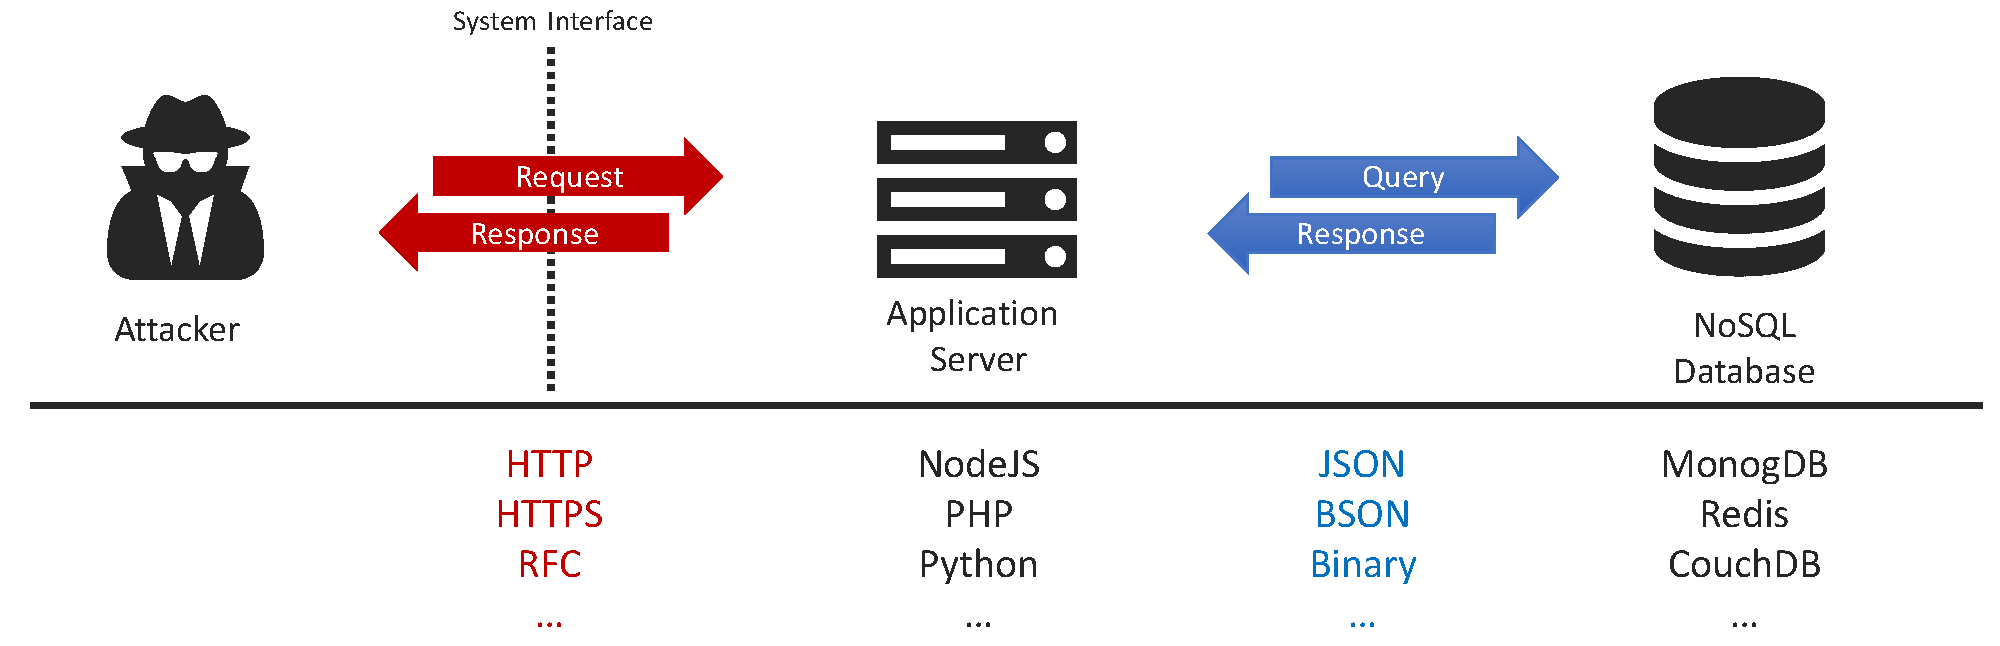
\includegraphics[width=1\linewidth]{Images/attacker_model_normal}
  \caption{Common attacker model for NoSQL injection}
  \label{fig:normalAttackerModel}
\end{figure}

% Objective

\subsection{Extended Attacker Model}

\begin{figure}[h]
\centering
  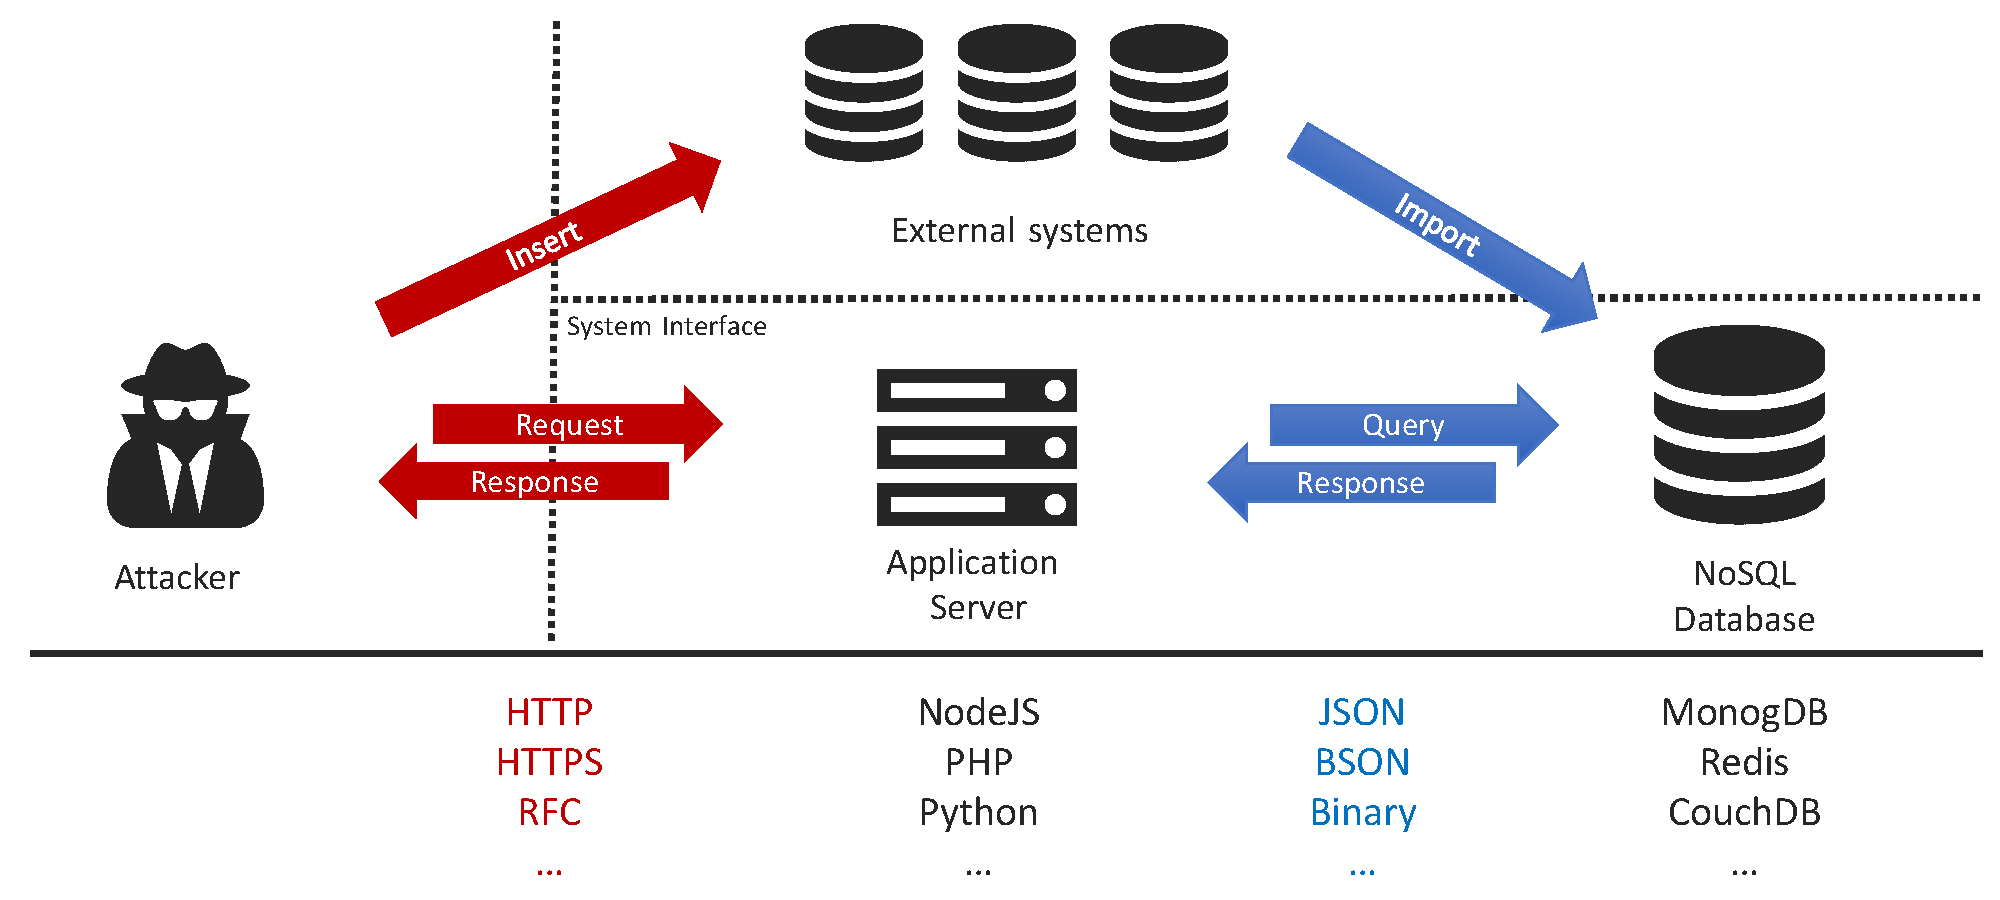
\includegraphics[width=1\linewidth]{Images/attacker_model_extended}
  \caption{Extended attacker model for NoSQL injection}
  \label{fig:extendedAttackerModel}
\end{figure}

% Objective

\subsection{Direct Attacker Model}

The deployment of RESTful interfaces allows a direct access from the client, omitting any application layer. Databases such as CouchDB explicitly refer to this architectural style for a simpler application design.

\begin{figure}[h]
\centering
  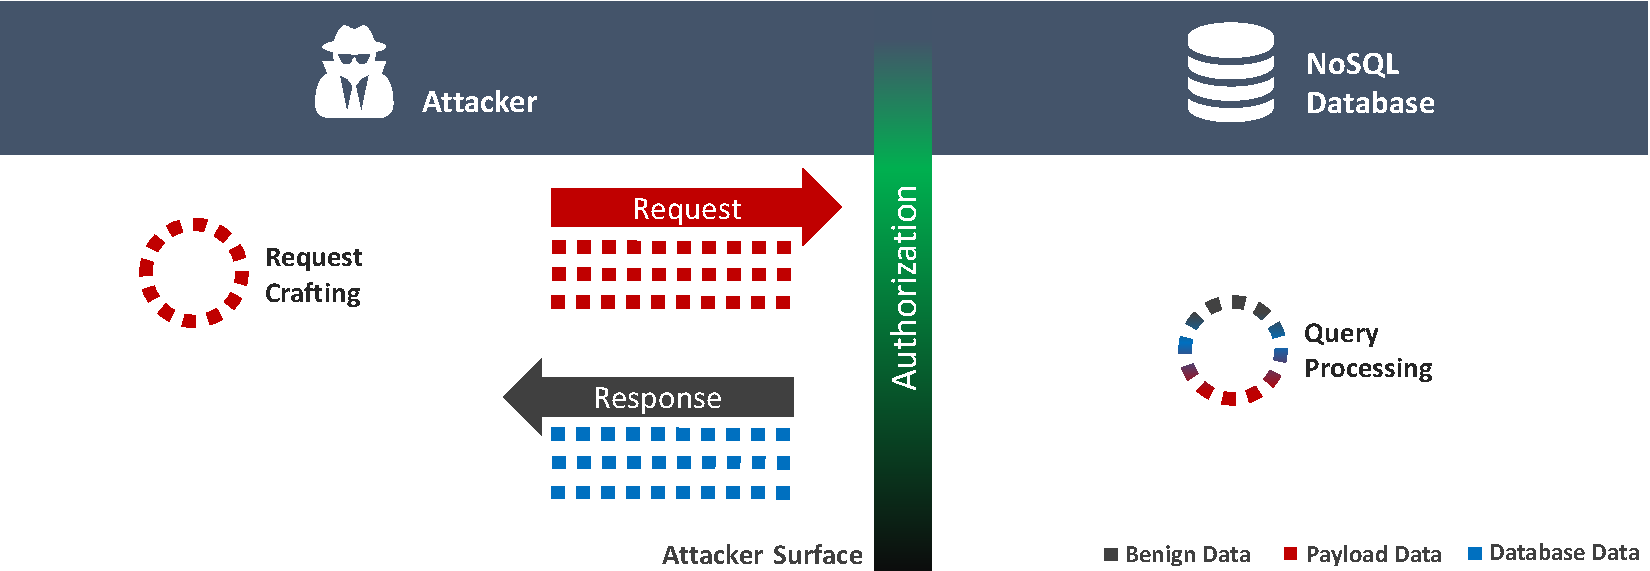
\includegraphics[width=1\linewidth]{Images/attacker_model_direct}
  \caption{Direct attacker model for NoSQL injection}
  \label{fig:extendedAttackerModel}
\end{figure}

% Objective


\section{Considered Technology Stack}
\subsection{Selected Databases}
\subsection{Selected Application Platforms}
  \chapter{NoSQL Injection Attacks}
This chapter gives an overview of the in scope of this thesis found NoSQL injection attacks. Each of the presented attacks is accompanied by a vulnerable code example as well as a suitable attack vector. With regard to the attacker surface parameters analyzed in section \ref{sec:analysisOfQueryTechniques}, the vectors focus on query string and JSON encoded payloads. The chapter is structured in one section per investigated database.

\section{MongoDB}
Within this section, the newly discovered injection attacks against the document store MongoDB are outlined.

\subsection{Query Selector Injection}
This attack is based on the Common Attacker Model and is directed against the selection parameter of queries. MongoDB employs BSON, an extended JSON format, to define the selected documents affected by the query. Complex selection operations, such as \textit{greater than} or \textit{not equal}, are implemented with the help of a set of special query selectors. These are formatted as objects and replace the actual value within the query criteria as demonstrated in listing \ref{lst:MongoQuerySelectors}. 

\begin{lstlisting}[caption={Example for MongoDB's query selectors}, label={lst:MongoQuerySelectors}]
find({'password' : 'secure'});      // Password property equals "secure"
find({'password' : {'$ne': '0'}});  // Password property not equals "0"
\end{lstlisting}

The injection attack presented by Sullivan \cite{Sullivan:2011} showed, that query selectors in combination with PHP applications can be utilized for injection attacks. Listing \ref{lst:PHPQuerySelectorInjection} shows the according vulnerable code of an login implementation. \\

\begin{lstlisting}[caption={Vulnerable PHP example for query selector injection on MongoDB}, label={lst:PHPQuerySelectorInjection}]
$collection->find(array('user' => $_GET['user'], 'password' => $_GET['password']));
\end{lstlisting}

The code checks for documents, that match the passed user and password values from the query string. Here comes the automatic query string parsing of PHP into play. This feature enables the injection of a Query Selector instead of an actual password with the help of the extended query string syntax. An passed selector like \textit{no equals} will nearly always evaluate to true. With the manipulated request shown in \ref{lst:QuerySelectorInjectionVector}, the login check can be reliably bypassed. \\

\begin{lstlisting}[caption={Attack vector on MongoDB for query selector injection via the query string parameter}, label={lst:QuerySelectorInjectionVector}]
https://example.org/login?user=patrick&password[%24gt]=
\end{lstlisting}

Pektov \cite{Petkov:2014a} demonstrated a vulnerable login implementation running on NodeJS's \textit{Express} web server following the same approach. The application code given in listing \ref{lst:NodeQuerySelectorInjection} can also be attacked with the request presented in listing \ref{lst:QuerySelectorInjectionVector} . \\

\begin{lstlisting}[caption={Vulnerable NodeJS example for query selector injection on MongoDB}, label={lst:NodeQuerySelectorInjection}]
db.collection('users').find({"user": req.query.user, "password": req.query.password});
\end{lstlisting}

So are there even any new findings for this class of attack? The previous publications presented the query selector injection as a distinct issue occurring only for PHP and Node applications, since its based a non-standardized application layer behavior. As explained in section \ref{sec:analysisOfQueryTechniques}, the query string parsing is a convenience functionality present across all investigated application platforms. The examples given in listing \ref{lst:RubyQuerySelectorInjection} for Ruby as well as listing \ref{lst:PythonQuerySelectorInjection} reveal, that query selector injection is an issue appearing across platforms. \\

\begin{lstlisting}[caption={Vulnerable Ruby example for query selector injection on MongoDB}, label={lst:RubyQuerySelectorInjection}]
db['users'].find({:user => req.params['user'], :password => req.params['password']})
\end{lstlisting}

\begin{lstlisting}[caption={Vulnerable Python example for query selector injection on MongoDB}, label={lst:PythonQuerySelectorInjection}]
db.users.find({"user": request.GET['user'], "password": request.GET['password']})
\end{lstlisting}

In all of the four cases, the default and by MongoDB recommended database driver was deployed. The attack vector from listing \ref{lst:QuerySelectorInjectionVector} leads in each of the presented login checks to the query criteria shown in listing \ref{lst:QuerySelectorCriteria}. \\

\begin{lstlisting}[caption={Resulting query of query selector injection}, label={lst:QuerySelectorCriteria}]
{'user': 'patrick', 'password': {'&gt':''}}
\end{lstlisting}

A login can therefore be bypassed in each investigated case, but this kind of attack is not restricted to login applications. Nearly all parameterized selection criteria can be influenced by the injection of query selectors. This includes all read, update and delete calls making use of the BSON selection format. Furthermore, the attacker surface analysis from section \ref{sec:analysisOfQueryTechniques} suggests, that the URL query string is by far not the only part of the attacker surface allowing this kind of attack. When the application processes other request parameters, the payload can also be placed in form data encoded as well as JSON request bodies. These circumstances exhibit a way more significant surface for query selector injection as previously indicated. \\


\begin{table}[h]
 \sffamily
 \centering
 \begin{tabular}{lll}
  \textbf{Command} & \textbf{Arguments} \\ \hline
  db.collection.deleteOne         & \textbf{filter} options \\
  db.collection.deleteMany        & \textbf{filter} options \\
  db.collection.find              & \textbf{query} projection \\
  db.collection.findAndModify     & \textbf{query} options \\
  db.collection.findOne           & \textbf{query} projection \\
  db.collection.findOneAndDelete  & \textbf{filter} options \\
  db.collection.findOneAndReplace & \textbf{filter} replacement options \\
  db.collection.findOneAndUpdate  & \textbf{filter} update options \\
  db.collection.replaceOne        & \textbf{filter} replacement options \\
  db.collection.remove            & \textbf{query} option \\
  db.collection.update            & \textbf{query} update options \\
  db.collection.updateOne         & \textbf{filter} update options \\
  db.collection.updateMany        & \textbf{filter} update options \\
  \bottomrule 
 \end{tabular}
 \caption{MongoDB commands affected by query selector injection}
 \label{tab:redis_commands_affected}
\end{table}

\subsection{Expanding Array Injection}
The expanding array injection is based on the common attacker model and exploits a special behavior of a query's selection criteria. When a requires a property to be equal to a value and the stored document contains an array in place of the property, all values of the array are used to find a match. This feature, as the attack name implies, is called automatic array expanding. An attacker can manipulate inserted documents in order to achieve matches subsequent selective criteria. The creation of an user as shown in listing \ref{lst:NodeJSCreateUser} represents an example for such an vulnerability. \\

\begin{lstlisting}[caption={Example for vulnerable MongoDB - NodeJS application}, label={lst:NodeJSCreateUser}]
if (req.query.user !== "admin") {
  db.collection('users').insert({"user": req.query.user, "password": req.query.password});
}
\end{lstlisting}

The given code allows the insertion of new users into the database, with the exception of \textit{admin} as a username. This security check can be bypassed, by injecting an array of usernames instead of a simple string. A suitable attack vector based on query string encoding is given with listing \ref{lst:ExpandingArrayInjection}.\\

\begin{lstlisting}[caption={MongoDB injection with NodeJS's query string module}, label={lst:ExpandingArrayInjection}]
https://example.org/register?user[]=patrick&user[]=admin&password=1234;
\end{lstlisting}

The given request creates an array typed \textit{user} property that leads to the bypass of the if-clause. In the next step, the query is executed and the provided data results into the document presented in listing \ref{lst:ExpandingArrayInjectionDocument} stored within the user collection.\\

\begin{lstlisting}[caption={Injected query parameter for MongoDB - NodeJS injection}, label={lst:ExpandingArrayInjectionDocument}]
{'user': ['patrick', 'admin'], 'password': 1234}
\end{lstlisting}

At this point, the array expanding functionality becomes important. An attacker can now use the normal authentication with username and password as shown in listing \ref{lst:NodeJSArrayExpandingLogin} to login. This works for both of the users inserted with the initial request. \\

\begin{lstlisting}[caption={Example for vulnerable MongoDB - NodeJS application}, label={lst:NodeJSArrayExpandingLogin}]
db.collection('users').find({"user": req.query.user, "password": req.query.password});
\end{lstlisting}

The request for the login, does have to be manipulated. An attacker can now login as an amdin with a usual authentication request as shown in listing {lst:ArrayExpandingAdminLogin}.\\

\begin{lstlisting}[caption={MongoDB injection with NodeJS's query string module}, label={lst:ArrayExpandingAdminLogin}]
https://example.org/login?user=admin&password=1234;
\end{lstlisting}

MongoDb will search for a document with the user property set to \emph{admin} and the password property set to \emph{1234}. Through the expansion the the beforehand injected document or respectively the user property, a matching document is found and the admin login is successful.\\

The presented login application is of course not the only example, where the expanding array feature of MongoDB allow injection attacks. Every insert operation with data originating from the three parameters, that allow type manipulation represents a potential vulnerability. It enables an attacker to break the confidentiality of the underlying data, which leads to unintended matches for further requests. The attack was exemplified for the NodeJS, but is relevant for all of the investigated application layers. 

\definecolor{dark-blue}{RGB}{0, 35, 71}
\definecolor{dark-red}{RGB}{120, 0, 0}
\begin{table}[h]
 \sffamily
 \centering
 \begin{tabular}{lllll}
  \textbf{Command} & \textbf{Arguments} \\ \hline
  db.collection.insert            & \multicolumn{3}{l}{\textcolor{dark-red}{\textbf{document}} | [ \textcolor{dark-red}{\textbf{document ... }} ] } \\
  db.collection.insertOne         & \textcolor{dark-red}{\textbf{document}} \\ 
  db.collection.update            & \textcolor{dark-blue}{\textbf{query}} \textcolor{dark-red}{\textbf{update}} options \\
  db.collection.updateOne         & \textcolor{dark-blue}{\textbf{filter}} \textcolor{dark-red}{\textbf{update}} options \\
  db.collection.updateMany        & \textcolor{dark-blue}{\textbf{filter}} \textcolor{dark-red}{\textbf{update}} options \\
  db.collection.replaceOne        & \textcolor{dark-blue}{\textbf{filter}} \textcolor{dark-red}{\textbf{replacement}} options \\\hline
  db.collection.deleteOne         & \textcolor{dark-blue}{\textbf{filter}} options \\
  db.collection.deleteMany        & \textcolor{dark-blue}{\textbf{filter}} options \\
  db.collection.find              & \textcolor{dark-blue}{\textbf{query}} projection \\
  db.collection.findAndModify     & \textcolor{dark-blue}{\textbf{query}} options \\
  db.collection.findOne           & \textcolor{dark-blue}{\textbf{query}} projection \\
  db.collection.findOneAndDelete  & \textcolor{dark-blue}{\textbf{filter}} options \\
  db.collection.findOneAndReplace & \textcolor{dark-blue}{\textbf{filter}} replacement options \\
  db.collection.findOneAndUpdate  & \textcolor{dark-blue}{\textbf{filter}} update options \\
  db.collection.remove            & \textcolor{dark-blue}{\textbf{query}}  option \\
  \bottomrule 
 \end{tabular}
 \caption{MongoDB commands affected by expanding array injection}
 \label{tab:redis_commands_affected}
\end{table}

\section{Redis}
This section covers the injection attacks against the key-value store Redis, that were found in scope of this thesis.

\subsection{Parameter Overwrite Injection}
The parameter overwrite injection against Redis is based on the common attacker model. It requires NodeJS as an application platform in combination with the most used Redis driver. In order to understand this attack, it is essential to know how parameters can be accessed to the this particular database driver. The regular way allows to pass each parameter as distinct argument. An alternative way allows to pass all parameters within a single array as the first argument of the function call. With this knowledge and the control of the first argument, an attacker is able to overwrite the following arguments of an driver function call. An example application, where this becomes critical is shown in listing \ref{lst:parameterOverwriteApp}. \\

\begin{lstlisting}[caption={Vulnerable NodeJS example for parameter overwrite injection on Redis}, label={lst:parameterOverwriteApp}]
RedisClient.expireat(req.query.key, new Date("November 8, 2026 11:13:00").getTime());
\end{lstlisting}

This code makes use of the \textit{expireat} functionality to set the data for the deletion of an entry. In this particular case, the expire date of the entry behind the passed key is set to a date far in the future. The user can therefore only extend the life of an entry behind an arbitrary key, but not really influence the stored data in a negative way. This situation changes, when the second parameter can be overwritten. A conceivable attack could set the expire data to a time in the past. An request, that triggers exactly this operation is shown in listing \ref{lst:parameterOverwriteAtt}. \\

\begin{lstlisting}[caption={Attack vector on Redis for query selector injection via HTTP GET}, label={lst:parameterOverwriteAtt}]
https://example.org/expire?key[]=foo&key[]=1117542887
\end{lstlisting}

Given the the query string parameters, the resulting array will be passed as the first argument to the database call. The following parameter, containing the future time will be overwritten. Instead the injected timestamp passed with with the array in the first argument will be used. Since this timestamp lays in the past, the stored data behind the provided key will be deleted. This enables an attacker to delete arbitrary entries of the database! Similar to the presented attack on \textit{expireat}, there exist multiple other affected database commands. An excerpt of commands, that are vulnerable for parameter overwrite injection are listed within table \ref{tab:redis_commands_affected}. \\

\begin{table}[h]
 \sffamily
 \centering
 \begin{tabular}{lll}
  \textbf{Command} & \textbf{Arguments} & \textbf{Injection Description} \\ \hline
  Append  & key value       & Append a value to an arbitrary key\\
  DecrBy  & key decrement   & Decrement the integer value of a selected key \\
  Del     & key [key ...]   & Delete multiple selected keys at once \\
  Exists  & key [key ...]   & Check existence of multiple keys at once \\
  Expire  & key second      & Delete arbitrary key \\
  ExpireAt& key timestamp & Delete arbitrary key \\
  GetRange& key start end & Get entire content of key \\
  GetSet  & key value & Overwrite value of selected key \\
  IncrBy  & key increment & Increment the integer value of a selected key \\
  Move    & key db & Set destination database \\
  Rename  & key newkey & Set new key \\
  Set     & key value [expire] & Set arbitrary key-value data \\
  \bottomrule 
 \end{tabular}
 \caption{Redis commands affected by parameter overwrite injection}
 \label{tab:redis_commands_affected}
\end{table}

The investigation revealed, that many of the commands allow parameter overwrites and therefore corruption on of the underlying data. When the first key argument is controlled by an attacker, all following can be overwritten. These vulnerabilities enable an attacker to perform unintended insert, update or delete operations.

\section{CouchDB}
Within this section, the discovered injection attacks against the document store CouchDB are outlined.

\subsection{Special Key Injection}

\begin{lstlisting}[caption={Vulnerable NodeJS example for special key injection on CouchDB}, label={lst:PHPArrayInjection}]
function checkUser(user, password, callback) {
  nano.use('users').get(user, (err, res)=> {
    callback(res.password === paasword);
  });
}

checkUser(req.query.user, req.query.password, handleResult);
\end{lstlisting}

\begin{lstlisting}[caption={Attack vector on CouchDB for speical key injection via HTTP GET}, label={lst:PHPArrayInjection}]
https://example.org/login?user=_all_docs
\end{lstlisting}

\subsection{Array Key Injection}

\begin{lstlisting}[caption={Vulnerable NodeJS example for array key injection on CouchDB}, label={lst:PHPArrayInjection}]
function getDocument(key, callback) {
  if (key === "secret" || key[0] === "_") {
    callback("No access!");
  } else {
    nano.use('table').get(key, callback);
  }
}

getDocument(req.query.key, handleResult);
\end{lstlisting}

\begin{lstlisting}[caption={Attack vectors on CouchDB for array key injection via HTTP GET}, label={lst:PHPArrayInjection}]
https://example.org?key[]=secret
https://example.org?key[]=_all_docs
\end{lstlisting}

\subsection{URL Traversal Injection}

\begin{lstlisting}[caption={Vulnerable NodeJS example for URL traversal injection on CouchDB}, label={lst:PHPArrayInjection}]
function getDocument(key, callback) {
  nano.use('table').get(key, callback);
}

getDocument(req.query.key, handleResult);
\end{lstlisting}

\begin{lstlisting}[caption={Attack vectors on CouchDB for URL traversal injection via HTTP GET}, label={lst:PHPArrayInjection}]
https://example.org/get?key=_design/credentials/_view/user_password
\end{lstlisting}

\section{Memcached}
This section covers the injection attacks against the key-value cache Memcached, that were found in scope of this thesis.
\subsection{Array Key Injection}
  \chapter{Classification of NoSQL Injection Attacks}
\label{cha:classification}
This chapter analysis the found injection attacks and classifies them according to the underlying problem. In the course of this, four major issues were identified that cause injection vulnerabilities in non-relational databases. These classes are outlined in the following sections with reference to the corresponding attacks of the previous chapter.

\section{Object Structure Defined Semantic}
With the emergence of non-relational databases, JSON became a prevailing format for the storage of data records. The document stores MongoDB and CouchDB are prominent examples for JSON-structured data persistence. Given this storage structure, utilizing the same format for query criteria suggested itself. The JSON-format allows to state property-value combinations that have to be match the stored data. For more complex query criteria, the JSON format has to be extended. The investigated document stores achieve this with objects that contain special keys. This structure represents a comprehensible notation for humans and mirrors the stored data records. In theory, also other formats could be applied instead of JSON. A query's semantic is therefore defined by the structure and properties of its parameters. As known from other query languages, the semantic defining elements have to be protected from injection attacks. In the case of SQL injection, these semantic defining elements are special characters of a string. For the investigated document stores, the semantic is encoded in the object structure of parameters. On account of this, the type and structure of user-provided values have to be validated. Without suchlike sanitizing, the parameter structure and type can be changed by injection attacks. Unfortunately, awareness of potential object structure and type injection is not very widespread. Restricting user-provided data to strings or integer values does not represent a feasible solution, since flexibility of parameters is required to work with unstructured data. A case differentiation between sensitive and benign parameter structures is needed. This differentiation has to be accomplished within the application layer since the sensitivity of parameter highly depends on the intended use case. Authentication or authorization operations are highly sensitive, whereas operations on public data are rather harmless. The required case differentiation exhibits a conceptual problem of the query technique regarding injection attacks.\\

This class of attacks was exposed by the results of the preceding investigation. The query selector injection against MongoDB as well as the find selector injection against CouchDB are based upon this conceptual issue. The problem has to be solved by proper structure and type sanitizing depending on the intended use case.

\section{Diverging Parameter Handling}
This class of attacks rests upon differences in the handling of parameters between application and database layer. These differences are crucial since the concept of non-relational databases depends on application layer data checks. Reasons for the differences can be automatic format or type conversions within the database layer and driver. Two diverging parameters may be converted to the same value and therefore result in the same database operation. An example could be an array that is automatically split into its components. This leads to multiple parameter combinations that trigger the same database operation due to the preliminary conversion. Before the conversion, the diverging parameters lead to varied behaviour of the application layer processing. Prevention of disallowed database operations by application layer checks becomes hard to ensure since multiple parameter combinations exist for a distinct operation. Such diverging handling of parameters is often not documented and therefore hard to consider within the application layer code. The underlying reason for the problematic conversions can be conceptual issues as well as implementation flaws.\\

The previous investigation exhibited multiple examples that lead to this class of attacks. Practical instances for this class of attacks are the expanding array injection against MongoDB, where elements of stored arrays are automatically extracted for comparison. The array value injection against CouchDB as well as the array key injection against Memcached automatically retrieve elements from arrays when another value type is required for the operation. Redis's parameter overwrite injection allows two ways to pass arguments and converts them within the database driver. The problem has to be solved by proper structure and type sanitizing within the application layer since these attacks rely on data type conversions.

\section{Shared Scope for Data}
Another class of injection attacks of non-relational databases is caused by shared storage scopes for multiple purposes. A storage scope can be seen as a delimited database section, such as a table or collection. Normally, data from different applications is stored in separate scopes. This situation changes with non-relational databases. The support for unstructured data enables the storage of various data formats within a single scope. This capability may be used by applications or the database itself to combine varied information within a single scope. An example is the storage of meta information next to normal data records within a single scope. In order to handle this correctly, the application layer has to be aware of the variety of formats. Since the concept of shared storage scopes is relatively new, many applications may only expect a single format within a storage scope. Other formats are therefore not considered within the application layer and may lead to unexpected data processing. Attacks of this class make use of this situation by manipulating queries in order to retrieve or insert unexpected data formats. For known attacks, this class is based on the conceptual design of the underlying database. \\

The investigation of the selected databases showed that shared storage scopes are actually employed. CouchDB stores meta data as documents within the corresponding collections. This results in data records that are accessible for each user on each collection by default. When these meta data records are not considered within the application layer processing, unintended behaviour can be triggered through query injection. The special key injection against CouchDB proves that such attacks can be critical. A shared storage scope also plays an important role for the data import injection affecting CouchDB. Thereby, mixed data formats within a single collection allow the execution of user-controlled JavaScript functions.

\section{Error-prone String Escaping}
The last class of attacks against NoSQL databases encompasses a problem already known from its relational counterparts. Concatenation of strings with user-provided parameters has to be approached with caution. As known form SQL, each untrusted string has to be escaped for the intended target context. This rule does not only apply to SQL but to all strings interpreted within the database layer. The new generation of non-relational databases employs various scripting languages and string parameters, whose parameters have to be properly sanitized. User-controlled data should never be in control of the semantic structure of such strings. Therefore, all control characters of the targeted context have to be escaped. Missing or incomplete escaping enables an attacker to manipulate the semantic of the later-on interpreted string. The described problem applies to all strings with a dedicated structure that are interpreted within the database layer. \\

This class of injection attacks is already known, but applies to a variety of contexts regarding non-relational databases. Mitigation techniques for this kind of problem exist, but the findings of this thesis imply that missing or error-prone parameter escaping still represents a severe problem. The targeted contexts changed, but the underlying problem is still the same. URL traversal injections, as found for CouchDB, belong to this class of error-prone string escaping. Other studies discovered multiple of this problems with regard to map-reduce function injection. This class compromises string defined semantics and therefore represents the counterpart to the first class that attacks object structure defined semantics.\\

\section{Classification Overview}
This section summarizes the previous attack classification and gives an overview of the underlying design problems. Table \ref{tab:attack_classification_overview} assigns each attack of the previous chapter to a distinct class. \\

\begin{table}[h]
  \sffamily
  \centering 
  \begin{tabular}{lll}
  \textbf{Class} & \textbf{Attack} & \textbf{Database} \\ \hline
  \multirow{2}{*}{Object Structure Defined Semantic}
    & Query Selector Injection & MonogDB \\
    & Find Selector Injection & CouchDB \\ \hdashline
  \multirow{4}{*}{Diverging Parameter Handling}
    & Expanding Array Injection & MonogDB \\
    & Parameter Overwrite Injection & Redis \\
    & Array Value Injection & CouchDB \\
    & Array Key Injection & Memcached \\ \hdashline
  \multirow{2}{*}{Shared Scope for Data}
    & Special Key Injection & CouchDB \\
    & Data Import Injection & CouchDB \\ \hdashline
  \multirow{1}{*}{Error-prone String Escaping}
    & URL Traversal Injection & CouchDB \\ \hline
  \end{tabular}
  \caption{Classification overview of the found injection attacks according to the underlying problem}
  \label{tab:attack_classification_overview}
\end{table}

The table shows that the new approach of object structure defined semantic leads to serious problems. Automatic parameter conversion within the database layer leads to diverging parameter handling and injection vulnerabilities across all investigated databases. Shared scopes for data storage are only present in case of CouchDB, but also expose a threat for injection attacks. Even the well-known problem of error-prone string escaping represents still a major issue for certain contexts, such as REST URLs. With the given classification of all found injection attacks and analysis of the according design problems, the in section \ref{sec:objective} set \textbf{objective 3} is covered.
  \chapter{NoSQL Injection Mitigation}
Within this section, a mitigation approach for injection attack against non-relational databases is presented. Based on the previous attack analysis and classification, a new prevention concept is elaborated addressing the major design problems. Further, a feasible way for the implementation of the presented mitigation technique is outlined and empirically evaluated.

\section{Conception}
In order to create a mitigation concept for NoSQL injection, the exposed design problems have to be considered. The last chapter concludes four major issues, that lead to injection vulnerabilities of non-relational databases. Since error-prone string escaping is a well-known and actually problem, the fourth class is not focused. The main issue brought along with non-relational databases is object structure defined semantic. This feature gives a raise to attacks based on error-prone type and structure escaping as well as diverging parameter handling. As exposed by the found attacks, problems of this kind are spread across all investigated databases and application layers. The third class of attacks is bases on shared storage scopes and is only present for CouchDB. This issue can be solved by strict data separation. Therefore, the main goal for attack mitigation is the prevention of type and object structure injection. This addresses two-thirds of the found injection attacks and represents a problem not adequately solved yet. \\

The first idea regarding the mitigation of type and object structure based injection attacks, may be simple type casting of parameters. Although, this strict method would prevent most attacks, it has major drawbacks. On the one hand, the required type casting is highly dependent on the use case and performed query. With this technique, developers are responsible for attack mitigation by applying suitable type castings for each query parameter. This resembles the idea of manual parameter escaping for SQL statements, which was not reliably applied by developers. A vital argument against type casting, is the flexibility required by many applications. Listing \ref{lst:ExampleFindQueryStringID} and \ref{lst:ExampleFindQuerySpecialID} exemplify a use case, that employs two different types of identifiers. \\

\begin{minipage}{.97\textwidth}
\begin{minipage}[t]{.49\textwidth}
\begin{lstlisting}[escapechar=!, caption={Example for find query with a string identifier}, label={lst:ExampleFindQueryStringID}]
db.find({
  "_id": !\textbf{"56767834"}!

});
\end{lstlisting}
\end{minipage}
\hfill
\begin{minipage}[t]{.49\textwidth}
\begin{lstlisting}[escapechar=!, caption={Example for find query with a special object identifier}, label={lst:ExampleFindQuerySpecialID}]
db.find({
  "_id": {
    !\textbf{"\$oid": "54651022bffebc03098b4567"}!
});
\end{lstlisting}
\end{minipage}
\end{minipage}

The given queries work on a database, that contains documents with varying identifier formats. Some documents use a string based identifier, others employ an object-based identifier. The latter type is used in order to indicate a special format of the stored identifier string. Such differences of data types are typical for non-relational databases, due to their ability to handle unstructured data. The highlighted parts of the code have to be under user control, to allow generic querying of both identifier types. In contrast to the given scenario, such querying becomes arbitrary complex depending on the number of different property types within the database. Type casting for the highlighted parameter can therefore not be applied. In summary, some use cases require structural control of user-provided query parameters. \\

So why not apply type casting of parameters where possible and otherwise grant full flexibility? Regarding the example given with listing \ref{lst:ExampleFindQueryStringID} and \ref{lst:ExampleFindQuerySpecialID}, query selector injection is still an issue. Therefore, the full flexibility has to be restricted a bit. At this point, the mitigation approach of this thesis applies. In order to grant a certain degree of flexibility, but still prevent injection, allowed parameter structures have to be defined for each query. Based on the requirements, this thesis suggest a pattern-based control mechanism for query parameterization. The patterns define a range of allowed query structures and the all others are blocked. This approach applies directly at the connection between application and database layer, within the database driver. Therefore, each input for the query can be reliably filtered without any danger of subsequent manipulation. \\

The presented approach still requires manual pattern definition for each query, but in contrast to type casting at least allows some kind of flexibility for query parameters. This idea can be taken a step further to bring another important advantage. The creation of the applied security patterns can be automatized. Basically, the idea is to learn the patterns in a secure execution environment of the application. In a second step, the application goes live and the pattern validation is activated. This can be seen as a learning and an execution phase. Software tests are normally present for each application and constitute a great means to build the security patterns based on trusted inputs. By providing such a framework, a solution independent from the underlying technology stack, concrete security patterns and implementation details is given. This approach provides the needed flexibility, does not require high engineering efforts and provides sufficient protection from the found injection attacks.

\section{Implementation}
The previously described mitigation technique for NoSQL injection attacks has to be transformed into practice. For the exemplary implementation outlined within this section, the most prevalent technology stack was selected. According to the statistics shown in chapter \ref{cha:intro_to_nosql_injection}, MongoDB and NodeJS represent the most widespread technologies relevant in scope of this thesis. As exposed by the initial investigation, this combination of application and database layer reveals severe weak spots for injection attacks. Therefore, an exemplary implementation of the presented mitigation technique is given for NodeJS applications running on MongoDB. \\ 

To stop object structure and type injections, all affected query parameters have to be sanitized. The most reliable way to accomplish this sanitizing, is an integration of the mitigation technique directly into the database driver. In avoidance of writing an entirely new database driver, the existing MongoDB driver for NodeJS is used and wrapped with an additional layer. The rough architecture and functioning of the implementation is visualized by figure \ref{fig:architecture_secure_driver}. \\

\begin{figure}[h]
\centering
  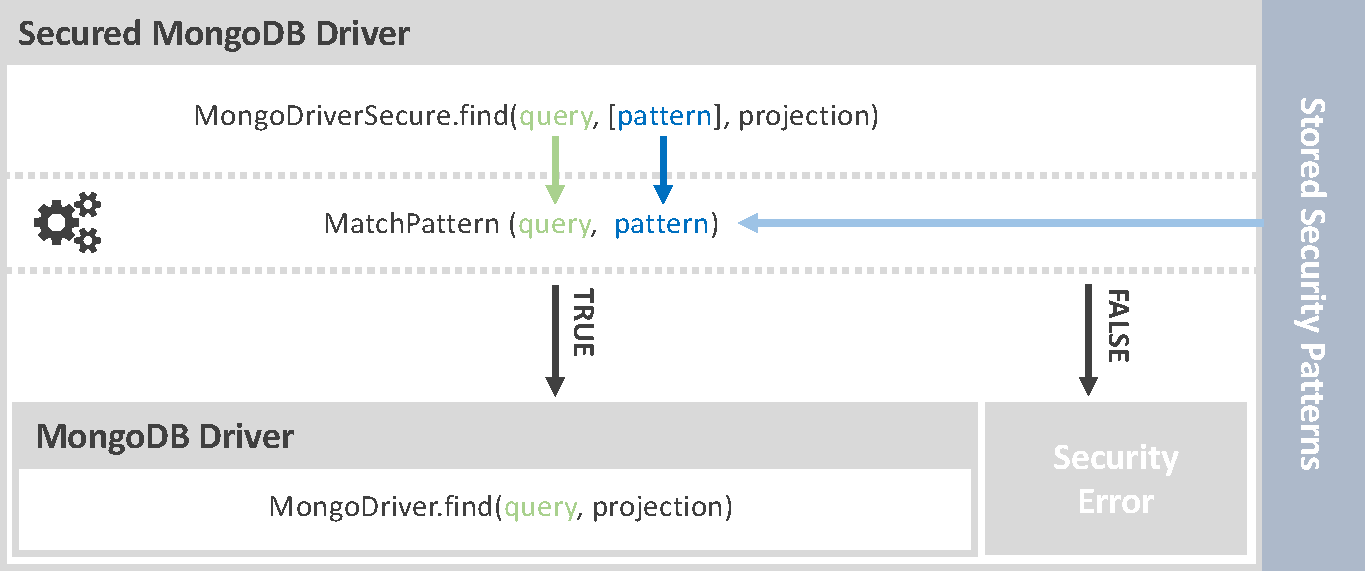
\includegraphics[width=1\linewidth]{Images/secure_driver}
  \caption{Architecture for the implementation of the NoSQL injection mitigation concept}
  \label{fig:architecture_secure_driver}
\end{figure}

Basically, the secured driver extends the former interface with optional \emph{pattern} arguments. These follow can be passed after the sensitive argument and define the allowed data types and structures. The shown example extends the find function with an optional security pattern for the \emph{query} argument. When no security pattern is provided by the arguments, the driver can alternatively draw on stored ones. These stored security patterns can be created automatically within a secure execution environment. In order to prevent injection, the extended driver matches the given security pattern with the passed argument. When both are compatible, all arguments except of the security patterns are forwarded to the normal MongoDB driver. Otherwise, a security error is thrown, that indicates a potential injection attack. In case no security pattern is provided, the query parameter are passed without further control to the wrapped driver. This behaviour enables a drop-in replacement of the secured driver without breaking any application. Similar to this implementation, drivers for other databases and application layers can be wrapped. \\

At this point, the employed security pattern structure has to be defined. There exist various possible ways to implement the patterns for the presented mitigation approach. This thesis proposes a JSON-based format for straightforward handling across all feasible application layers. Listing \ref{lst:security_pattern_grammar} shows the grammar of the security patterns used for the outlined implementation. \\

\begin{lstlisting}[escapechar=!, caption={Proposed security pattern grammar for the injection mitigation mechanism}, label={lst:security_pattern_grammar}]
<SecurityPattern> ::= {'_security_pattern': <Option> };
<Options> ::= <Option> | <Option>, <Options>;
!\textbf{<Option> ::= [<Values>]}!;
<Value> ::= <Array> | <Object> | <Type>;
<Array> ::= [] | [!\textbf{<Options>}!];
<Object> ::= {} | {<Properties>};
<Values> ::= <Value> | <Value>, <Values>;
<Properties> ::= <Property> | <Property>, <Properties>;
<Property> ::= <Key> : !\textbf{<Option>}!;
<Type> ::= "String" | "Number";
<Key> ::= *Arbitrary String*;
\end{lstlisting}

The given grammar for the security patterns resembles the one of JSON. On the top level, the \emph{\_security\_pattern} property is fixed, to be able to distinguish normal and pattern arguments. Furthermore, each value of objects and arrays is replaced by an option array as highlighted. This allows the declaration of multiple allowed types and structures and ensures the required flexibility. The options array in turn contains other structures or type definitions. In order to keep the grammar neat, the last rule for arbitrary key strings is shortened. Strings and numbers are indicated with the according string, arrays an objects are represented by the actual JSON elements. Since this may be hard to imagine, a practical example is given within listing \ref{lst:security_pattern_example_id}. \\

\begin{lstlisting}[escapechar=!, caption={Security pattern allowing string-based and object-based identifiers as a query parameter}, label={lst:security_pattern_example_id}]
{"_security_pattern_": [{
  "_id": ["String", {"$oid": ["String"]}]
}]}
\end{lstlisting}

This security pattern is tailored to the motivational example given by listing \ref{lst:ExampleFindQueryStringID} and \ref{lst:ExampleFindQuerySpecialID} in the previous section. Two alternatives are listed for the \emph{\_id} property. Either a string value can be passed or an object containing a string-based property with the key \emph{\$oid}. The pattern can be passed as an additional parameter to the secured MongoDB driver or created with the help of exemplary queries. Thereby, the advantage of the options array for automatic pattern learning becomes clear. For each observed query that is not covered by the pattern, an additional option can be appended to the array. \\

The implemented driver is published as an open source project and can be installed via the Node Package Manager. \textbf{(https://www.npmjs.com/package/mongodb-secure)}


\section{Evaluation}
\label{sec:evaluation}
Within this section, the designed mitigation technique for NoSQL injection is evaluated by means of the outlined implementation. First, the applied methodology is explained and afterwards, the evaluation results regarding compatibility and security are summarized.

\subsection{Methodology}
In scope of this evaluation, two major aspects of the injection mitigation technique have to be considered. The first one is the compatibility of the implemented solution with existing applications. A mitigation approach, that requires high engineering efforts and code changes to be compatible, would not be viable in practice. The other aspect is the provided security form injection attacks against the underlying database. This security aspect has to be evaluated with regard to the addressed attack classes. \\

In order to give an empirical evaluation, a group of open source applications is selected. These applications have to be built with NodeJS and MongoDB, to allow the integration of the implemented secure driver. To enable the required driver integration, the code of the selected applications has to be public accessible. Based on this criteria, the following widespread projects were selected for the further evaluation.

\begin{description}
\item [Agora] This project is developed by the German Softwerkskammer and builds the central platform for their communities. ({\footnotesize\url{https://github.com/softwerkskammer/Agora}})
\item [Apostrophe 2] With the goal of an design-driven and flexible content management system, Apostrophe bets on NodeJS and MongoDB for its most current version.\\
({\footnotesize\url{http://apostrophecms.org/}})
\item [Habitica] This project set its objective, to create a productivity enhancing and habit building application with the help of an integrated gamification concept. ({\footnotesize\url{https://habitica.com}})
\item [NodeBB] The goal of this platform is to deliver a powerful and mobile-ready forum software for the modern web. ({\footnotesize\url{https://github.com/NodeBB/NodeBB}})
\item [Pencilblue] This application represents an open source content management system for business class use cases. ({\footnotesize\url{https://pencilblue.org/}})
\end{description}

Next to the listed projects, also the original MongoDB driver for NodeJS is considered for the evaluation. The general approach is, to utilize the tests available for each of the applications. In a first step, these test are executed and the number of passed ones is measured. Then, the existing MongoDB driver is replaced with the secured one. The same tests are run again with the changed setup and the number of passed ones is again measured. Thus, the measured ratios of passed test can be compared for each application. With regard to the security aspect, it represents a problem to find an appropriate measurement. The mitigation of real world vulnerabilities would be a feasible approach, but these are not available in scope of this work. Therefore, the guarantees given by the new driver implementation and the coverage of attack classes are evaluated.

\subsection{Compatibility}
The following measurements were performed with the normal as well as the secured driver, whereas the patterns allowed all feasible inputs. Automatic pattern learning was not conducted, since training and evaluation on the same test sets would deliver non-representative data. The described compatibility evaluation lead to the results, presented within table \ref{tab:compatbility_eva_overview}. 

\begin{table}[h]
  \sffamily
  \centering 
  \begin{tabular}{llrrr}
  \multirow{2}{*}{\textbf{Application}} & \multirow{2}{*}{\textbf{Type}} & \multicolumn{3}{c}{\textbf{Passed Tests}} \\ \cdashline{3-5}
    & & \textbf{Normal Driver} & \textbf{Secured Driver} & \textbf{Deviation}  \\ \hline
  MongoDB driver & Database Driver & 1047 & 1039 &  \cellcolor{light-gray} < 1\% \\
  Agora & Group-ware Platform & 1415 & 1415 & \cellcolor{light-gray}0\% \\
  Apostrophe 2 & Content Management System & 274 & 274 & \cellcolor{light-gray}0\%  \\
  Habitica & Habit Building Program & 2074 & 2074 & \cellcolor{light-gray}0\% \\
  NodeBB & Forum Software & 374 & 374 & \cellcolor{light-gray}0\% \\
  Pencilblue & Content Management System & 610 & 610 & \cellcolor{light-gray}0\% \\ \hline
  \end{tabular}
  \caption{Rate of passed tested with normal and secured MongoDB driver}
  \label{tab:compatbility_eva_overview}
\end{table}

Listed are the number of passed tests of both driver versions for each of the investigated applications. In addition, the interface test of the normal driver were also run with the secured version. The last column shows the relative deviation of passed tests from the secured driver in comparison with the normal driver. As highlighted, the added security layer breaks less than one percent of the database interface tests. A closer look revealed, that few tests fail because of missing dependencies. This problem originates from the new architecture and the surrounding wrapper, but does not represent an conceptual issue. With regard to the numbers measured with the selected applications, the secured driver shows no deviation at all. Test execution behaves exactly the same as with the default database driver. Therefore, the implemented mitigation technique can be integrated into existing applications without further engineering efforts. The secured driver replaces the normal one and enables developers to pass optional security pattern arguments. 

\subsection{Security}
The security provided by the mitigation technique integrated into the database driver is highly dependent on the underlying security patterns. It has to be emphasized, that the implemented driver does only provide protection, when security patterns are defined. This can happen through the additional query parameters or the approach of automatic pattern learning. Even when the security patterns are provided, the reliability of the mitigation approach still depends on the quality of the patterns. In case of pattern learning, the quality is influenced by the trusted environment. When during the learning phase not each possible query parameter format is covered, the false-positive rate of the execution phase will increase. On the assumption of perfect security patterns, all injection classes depending on object structure and type manipulation can be reliably prevented. Injection classes based on error-prone string escaping or shared data storage are not covered by the mitigation approach. \\

With the proposed mitigation technique for NoSQL injection and the promising evaluation results, a suitable solution for the in section \ref{sec:objective} set \textbf{objective 4} is given.
  \chapter{Evaluation}
\label{cha:Empirical Evaluation}
  \chapter{Related Work}
This chapter outlines related work and publications regarding NoSQL Injection attacks and prevention. First an overview of known NoSQL injection vectors is given and afterwards existing approaches for injection prevention are summarized. In doing so, similarities as well as the major differences in comparison to this thesis are discussed.

\section{NoSQL Injection}
Within this section, the publications of known NoSQL injection vectors are summarized in chronological order. Afterwards a comparison to the results of this thesis is given. \\

\textbf{Security - NoSQL-Injection}\cite{Oftedal:2010} \\
The presence of injection attacks on NoSQL databases was first demonstrated in a blog post by Erlend Oftedal in 2010. He described attacks on MongoDB based on string concatenation of parameters. In the process, BSON objects or JavaScript expressions are built with user controlled data and then passed to the database. In the former case the attacker is able to alter the BSON object structure and therefore the semantics of the query parameter. In the latter case, scripts, that are executed within the database, can be manipulated by an attacker. The behaviour of queries can be influenced in either case. \\

\textbf{Sever-side JavaScript Injection}\cite{Sullivan:2011} \\
In 2011 Brian Sullivan presented further NoSQL injection vectors as a part of a BlackHat session. Next to CSRF attacks on NoSQL databases and NodeJS security issues, he illustrated two attack vectors for NoSQL injections based on MongoDB and PHP. The structure of parameters is altered through a PHP feature called associative arrays. These allow a special syntax for URL-based query-strings that are then interpreted as arrays in PHP. As soon as query-string parameters are used as a part of database query parameters, arbitrary objects can be injected instead of string values. In combination with MongoDB's special keys, affected query criteria can be semantically manipulated. The second presented attack vector is executed in the same manner, but the special array key \textit{\$where} is used. As defined by the specification, MongoDB evaluates the value of this key as a script. Hence, a script injection for single query criterion can be performed. \\

\textbf{A Comparison: the Level of Security on Top 5 Open Source NoSQL Databases} \cite{Noiumkar:2014} \\
A general overview of the current state of NoSQL security was given by Noikumar et al. in 2014. They examined the most popular NoSQL databases - MonogDB, Cassandra, CouchDB, Hypertable and Redis - with regard to encryption, authentication, script injection and DoS attacks. MongoDB and CouchDB exposed possible script injections, whereas the other databases where classified as secure for this kind of attack. Other types of injection attacks, as presented within this work, were not considered. \\

\textbf{Hacking Node.js and MongoDB}\cite{Petkov:2014a, Petkov:2014b} \\
Injection attacks for MongoDB in combination with NodeJS were published by Petko Petkov on his web security blog in 2014 \cite{Petkov:2014a, Petkov:2014b}. With an example he illustrated, how to bypass a typical login implementation. Similar to the known PHP associative array injection, some major modules of NodeJS allow a special syntax to insert arrays from the URL's query-string. This in turn allows to alter query criteria by object injection. In the login case, a greater than comparison in contrast to the default equals comparison is inserted for the user and password value. As a result, both criteria are evaluated to true and the login is bypassed. In addition to the GET request based example, also a POST request version of his attack vector is shown. Within the second article, Petkov gave an example for his attack vector with realistic circumstances. By use of object injections, a brute-force attack for hashed passwords on all users is possible.\\

\textbf{The New Page of Injections Book: Memcached Injections} \cite{Novikov:2014} \\
Security researcher Ivan Novikov presented a technique for command injection attacks on Memcached on BlackHat in 2014. He showed how to append additional commands to existing queries. By the injection of special bytes such as newline characters, the actual command is terminated. Since these special bytes were not escaped, the database interpreted trailing characters as a new command. Multiple versions of this attack for Ruby, Python and PHP with corresponding database drivers were revealed by the publication. The injection vector is not based on a conceptual problem of the database, but frequent implementation flaws in the database drivers. \\

\textbf{No SQL, No Injection? Examining NoSQL Security} \cite{Ron:2015} \\
One of the latest publications covering NoSQL injection was release by Ron et al. in 2015. The paper gives an overview of NoSQL injection vulnerabilities across databases. Known injection vectors such as the associative array injection on MongoDB via PHP \cite{Sullivan:2011} and string concatenation of objects \cite{Oftedal:2010} were resumed. Additionally, the researchers published an example for a MapReduce injection on MongoDB that allows to execute scripts in scope of the database. This new attack vector works across application platforms and is based on concatenation of strings in order to build a map or a reduce function. Although MapReduce is called for specific collections of MongoDB, in this scenario the attacker is able to access and change data of other collections. Proposed mitigation approaches were the encoding of input data and dynamic application security testing.\\

As former publications show, NoSQL injection is also an existing issue in the new generation of databases. In the majority of cases, only single attack vectors for specific database and application platform combinations are presented. MongoDB is often focused by security research, since it is the most prevalent database. By contrast, other NoSQL databases are hardly considered and only few injection vectors are documented. With respect to the application layer, that is an important factor for attacks, usually only PHP and NodeJS are taken into account. This thesis addresses multiple prevalent NoSQL databases in combination with the most common application layers and drivers. Therefore, a comprehensive overview of NoSQL injection can be given. In contrast to former publications concentrating on single attacks, this thesis reveals NoSQL injections as an overall issue across platforms.\\

\section{NoSQL Injection Prevention}
Within this section, the publications covering approaches for NoSQL injection mitigation are summarized and afterwards compared to the solutions proposed by this work. \\

\textbf{Diglossia: detecting code injection attacks with precision and efficiency} \cite{Son:2013} \\
The 2013 published paper by Son et al. suggest a system for precise injection detection for SQL as well as NoSQL databases. They propose a dynamic analysis of user controlled data and showcase the idea with an adapted PHP interpreter and extended database parser. A taint-tracking system marks user and system controlled characters of strings. For database calls, a special parser checks the taint information of all input parameters. In case taint is contained in sensitive tokens, the query is terminated. Otherwise, the normal parser of the database is called. Attacks on the structure of query parameters can be reliably prevented with this approach.\\

\textbf{Analysis and Mitigation of NoSQL Injections} \cite{Ron:2016} \\
The latest publication on the mitigation of NOSQL injection was presented by Ron et al. in 2016. They describe the current-state of NoSQL injection as well as best-practices for attack prevention. Known injection vectors are classified as tautologies, union queries, piggybacked queries or JavaScript injections. In order to address the threats, guidelines for the entire software development life cycle are suggested. This involves three main tasks - development, testing and deployment. At the time of development, software design should be security driven, established libraries for validation and sanitation should be used and privileges should be clearly isolated. Static and dynamic security scanning as well as code reviews by security professionals should represent important parts of the testing process. In the next step, deployed software should be protected on network and API level. Finally, monitoring and intrusion detection systems should be applied. According to Ron et al., the relatively new security approach of self-protecting application runtimes represents an additional solution for NoSQL injection mitigation.\\

As previous publications show, NoSQL injection is a prevalent problem, that has to be addressed. Presented solutions may solve some of the injection vulnerabilities, but also bring along major drawbacks. Stricter development and software guidelines, as proposed by Ron. et al. \cite{Ron:2016}, may lead to fewer NoSQL injection vulnerabilities. However, these measures entail high efforts in developer training and software testing and still do not guarantee secure software. Systematic approaches, such as taint-tracking suggested by Son et al. \cite{Son:2013}, provide security for designated types of NoSQL injection attacks. Unfortunately, the strict constraints for untainted query structures restricts the essential flexibility of NoSQL databases. In order to combine this mitigation approach and data flexibility, application code has to handle much of the complexity. In addition, a taint-tracking system implicates higher memory consumption and thereby performance disadvantages. By contrast, only minor code changes are needed for the solution based on security-patterns demonstrated within this work. System performance is also not affected by the proposed solution and a clear scope for covered NoSQL injection types is given. Another improvement of the security-pattern in comparison to existing approaches is, that the concept can be applied in an adapted way to other databases with divergent injection types. All in all, the proposed prevention mechanism represents a more general and well scoped approach for NoSQL injection prevention.
  \chapter{Conclusion}
This final chapter discusses the results of this thesis with regard to the initially set objectives. Afterwards, an outlook for further research in scope of NoSQL injection is given.

\section{Discussion}
Injection attacks against non-relational databases represent a serious issue. System landscapes become more and more heterogeneous with direct impact on security. Therefore, existing attacker models for injection attacks have to be reconsidered. This work introduces two new attacker models next to the established one, known from SQL injection. These are required to deliver a clear definition for injection attacks against NoSQL databases. With the given definition and analysis of attacker models, the first objective of this thesis is covered. Based on this, the most prevalent technology stacks were selected for further investigation. The research in scope of this work revealed multiple new injection vectors across all selected databases and application layers. Two of the three attacker models - the normal and the extended one - were affected by actual attack vectors, whereas the direct attacker model stayed unconcerned. This proves that injection attacks against non-relational databases are not individual cases, like previous publications indicated. With the broad spectrum of investigated technology stacks, a holistic view of the subject is given for the first time. Thus, the second objective of this work is covered comprehensively. Likewise, the presented research broke down the found injection vectors and exposed multiple conceptual problems. This attack classification gives a clear overview of the faced challenges for NoSQL injection prevention. Especially, the new categories of object structure and type injections were not approached until now. In this way, the third objective set in scope of this work is addressed. Ensuing from the attack classification and requirements of non-relational databases, a mitigation approach was presented that considers flexibility, security and feasibility. As the empirical evaluation showed, the presented solution can be integrated into existing implementations without any problems. The generic approach provides an additional layer of security and compatibility across all investigated platforms, as the practical implementation proves. Therewith, also the fourth and last objective was successfully addressed. \\

All in all, NoSQL injection represent a more serious problem than expected thus far. This work demonstrated, that this class of attacks has to be considered with the entire technology stack in mind. The variety of injection vectors and classes of attacks also requires new approaches for a secure operation of non-relational databases. 

\section{Outlook}
NoSQL injection represents a relatively new class of attacks and offers a broad range for further research. This thesis examined the most relevant databases and application layers, but there exists a broad range of technology stacks not covered by investigation so far. Especially graph and column stores represent types of non-relational databases that are not addressed by research yet. An all-encompassing overview of the topic would be desirable. The immense amount of technology stacks constituted of application and database layers as well as applied frameworks and database drivers make an all-inclusive examination an ambitious challenge. Therefore, an important topic for further research is the classification of the underlying design problems. With the help of these classes, generic mitigation techniques against injection attacks can be developed and implemented across all platforms. The evaluated mitigation approach presented in scope of this thesis seems promising for the class of error-prone type checks. To deploy the idea in practice, further work on the security pattern learning and pattern matching has to be done. This is important to reduce false-positives in production and still guarantee the required flexibility. In general, the design of new approaches for injection mitigation constitutes a vital topic for further work. All in all, this thesis provides a holistic insight into the topic of NoSQL injection, but there is still a broad spectrum for the investigation of attacks and mitigation research. 

\end{onehalfspace}

% ---------------------------- Literaturverzeichnis ----------------------------------------------
\printbibliography

% ------------------------------- Anhang ---------------------------------------------------------
%\begin{appendix}
%\clearpage Appendix
%\end{appendix}

\end{document}